\documentclass{article}
\usepackage[left=3cm,right=3cm,top=2cm,bottom=2cm]{geometry} 
\usepackage{makeidx}         % allows index generation
\usepackage[pdftex]{graphicx,color}          % standard LaTeX graphics tool
\DeclareGraphicsRule{.pdftex}{pdf}{.pdftex}{}
                             % when including figure files
\usepackage{multicol}        % used for the two-column index
\usepackage[bottom]{footmisc}% places footnotes at page bottom

\usepackage{booktabs}
\usepackage{arydshln}
\setlength\dashlinedash{0.5pt}
\setlength\dashlinegap{1.5pt}
\setlength\arrayrulewidth{0.3pt}

\usepackage{amssymb}
\usepackage{amsmath}
\usepackage{pifont}
\usepackage{bm}
\usepackage{cancel}
\usepackage{multirow}
\usepackage{amsmath}
\usepackage{epstopdf}
\usepackage[caption=false,font=footnotesize]{subfig}


\DeclareMathOperator*{\argmin}{arg\,min}

\DeclareGraphicsExtensions{.eps, .pdf, .png, .jpg}
\graphicspath{{./images/},{./}}

\newcommand{\red}[1]{{\color{red}#1}}
\renewcommand{\vec}[1]{\bm{#1}}
\newcommand{\mat}[1]{\bm{#1}}
\newcommand{\cframe}[1]{$\langle #1 \rangle$}
\newcommand{\prescript}[2]{\phantom{}^{#1}_{#2}}

\newcommand\frontmatter{%
    \cleardoublepage
%%  \@mainmatterfalse
  \pagenumbering{roman}}
\newcommand\mainmatter{%
    \cleardoublepage
%%  \@mainmattertrue
  \pagenumbering{arabic}}
%%%%%%%%%%%%%%%%%%%%%%%%%%%%%%%%%%%%%%%%%%%%%%%%%%%%%%%%%%%%%%%%%%%%%

\begin{document}
\frontmatter
\onecolumn 
\vskip 1cm
%\pagestyle{empty}
\begin{center}
\huge \textsc{Cooperative Robotics}\\
\vskip 1cm

\skip 0.5cm

\vskip 5cm

\normalsize
Authors:  \hspace{7cm} Email: \\  
Dikshant Thakur \hspace{6.8cm} s5938924@studenti.unige.it\\
Ouassim Milous \hspace{7cm}  s5943225@studenti.unige.it\\
Girum Molla Desalegn \hspace{6cm} s6020433@studenti.unige.it\\
\vskip 13cm
Date: 02/02/2025 \\
\end{center}
\clearpage
\section{Exercise 1: Implement a Complete Mission}
Implement several actions to reach a point, land, and then perform the manipulation of a target object.

Initialize the vehicle at the position:
\begin{displaymath}
	\begin{bmatrix} 8.5 & 38.5 & -36 & 0 & -0.06 & 0.5 \end{bmatrix}^\top
\end{displaymath} 
Use a "safe waypoint navigation action" to reach the following position: 
\begin{displaymath}
	\begin{bmatrix} 10.5 & 37.5 & -38 & 0 & -0.06 & 0.5 \end{bmatrix}^\top
\end{displaymath} 
Then land, aligning to the nodule. In particular, the $x$ axis of the vehicle should align to the projection, on the inertial horizontal plane, of the unit vector joining the vehicle frame to the nodule frame.
Once landed, implement a ``fixed-based manipulation action'' to reach the target nodule (mimicking the scanning of the nodule). During this manipulation phase, the vehicle should not move for any reason.



\subsection{Q1: Report the unified hierarchy of tasks used and their priorities in each action.}

\noindent

$\mathcal{A}_{1}$ - Safe Waypoint Navigation Action. 


$\mathcal{A}_{2}$ - Nodule Alignment Action

$\mathcal{A}_{3}$ - Safe Landing Action

$\mathcal{A}_{4}$ - Fixed Base Manipulatin Action
\begin{table}[htb]
	\label{tbl:actions_tables}
	\begin{center}
		\footnotesize
		\begin{tabular}{cccccc}
			\toprule		
			Task & Type & $\mathcal{A}_{1}$ & $\mathcal{A}_{2}$  & $\mathcal{A}_{3}$  & $\mathcal{A}_{4}$ \\
			\midrule
			Minimum Altitude                    & I & 1 & 1 & 1 & 1  \\
			\hdashline
			Horizontal Alignment                & I & 2 &  & &  \\
			\hdashline
			Nodue Alignment                       & E &   &  & 2 & 2   \\
			\hdashline
			Landing 						& E & & 2 & & 3 \\
			\hdashline 
			Vehicle Stop 						& E & & & & 4 \\ 
			\hdashline 
			Tool Manipulatin					& E & 3 & & & \\
			\hdashline 
			Position Control 						& E & & & & 5 \\ 
			
			\bottomrule
		\end{tabular}
	\end{center}
\caption{Example of actions/hierarchy table: A number in a given cell represents the priority of the control task (row) in the hierarchy of the control action (column). The type column indicates whether the objective is an equality (E) or inequality (I) one.}
\end{table}
\\
Task Defintions\\
Minimum Altitude - This task maintains the altitude between vehicle and sea floor.\\ 
Horizontal Alignment - This task responsible to maintain the horizontal position with respect to sea floor. \\
Rock Alignment - This task is responsible to align the vehicle head with x axis of nodule. \\
Landing - This task is responsible to land the uvms system  on the sea floor. \\
Vehicle Stop - To make sure that vehicle will not move during the manipulation task. \\
Tool Manipulatin - This task move the manipulator arm to the goal position.\\
Position Control - It controls the vehicle to achieve its desired location.\\

\subsection{Q2: Comment the behaviour of the robots, supported by relevant plots.}
On the basis of the actions , which are mentioned above, we define our phases and here are our observation. 

Comment 1 - In the action of Safe Waypoint Navigation , vehicle starts from its intial position and goes linearly to its desired position. Keeping the vehicle horizontal stable and the manipulator is still not active. \\
PLOT OF THE GRAPH\\
Comment 2 - After reaches the desired position, whole system align itself with the x axis of nodule. Keeping the whole system horizontal stable.  \\
TOP VIEW\\
Comment 3 - In this phase, keeping the vehicle aligns with respect nodule x axis and sea floor, whole system goes to the sea floor vertically. 
PLOT THE GRAPH FOR ALTITUDE.\\
Comment 4 - Once the vehicle lands the manipulator arm will reach to the noduel, which is its desired position. 
\\PHOTO and PLOT

\subsection{Q3: What is the Jacobian relationship for the Alignment to Target control task? How was the task reference computed?}
To align the vehicle with the nodule, we calculated the angle difference between vehicle and nodule.
Here is the calculation step:
First we calculated the the distance between the current posiition and the nodule with respect to world frame.\\
$${}^{w}v_t = {}^{w}v_{goal} - {}^{w}v_{current} $$  %We should add the right mathematical formula
\noindent
With that distance vector, we find the angle between the current position of the vehicle and the target position of the vehicle with respect to world frame.\\
$${}^{w}v_t = {}^{w}v_{goal} - {}^{w}v_{current} $$ %Write in mathematical form. 
Once we have the angle difference then we constraint the yaw angular vehicle velocity in like this:\\
%Formula
$$\dot{x}_{yaw}=\psi_{taget}-\psi_{current}$$
The Jacobian we are using is the same we used in the vehicle posiition control task. Because we constrained our velocities only for yaw angular vehicle axis, so only solution we will get is for the yaw angular vehicle velocity. 
 %Jacobian formula
$${}^{w}J_v = \begin{bmatrix}
		\mathbf{0}_{3 \times 7} & \mathbf{I}_{3 \times 3} & \mathbf{0}_{3 \times 3} \\
		\mathbf{0}_{3 \times 7} & \mathbf{0}_{3 \times 3} & \mathbf{I}_{3 \times 3}
		\end{bmatrix} $$
\subsection{Q4: Try changing the gain of the alignment task. Try three different values: 0.001, 0.1, 1.0. What is the observed behaviour? Implement a solution that is gain-independent guaranteeing that the landing is accomplished aligned to the target.}
We observed that with gain 1.0, the time taken by vehicle to reduce the angular error between its body and nodule around z-axis with respect to world frame is faster than if we assign the gain 0.1 and 0.001. To be precise the time take in the first case, when gain is 1, is 10.5 seconds. In the second and third case, which are 0.1 and 0.001 respectively, it takes 52 seconds and in the latter case it moves infinitinemaly slow. 
%PLOT THE GRAPH

\subsection{Q5: After the landing is accomplished, what happens if you try to move the end-effector? Is the distance to the nodule sufficient to reach it with the end-effector? Comment the observed behaviour.}
After landing task, the manipulator easily achieved its task without vehicle moving. 

\subsection{Q6: Implement a solution that guarantees that, once landed, the nodule is certainly within the manipulator's workspace.}
To make sure that nodule is always in the work space of the manipulator arm. We need to control the vehicle in such a way it always come closer to the nodule.
For that first we need to calculate the x and y component of linear error, because we always activate this task after we have done the horizontal alignment, between the rock and tool. \\
%FORMULA
After getting the x and y component of linear error, we constrain our vehicle linear x and linear y velocities in such a manner:
%FORMULA

\clearpage
\section{Exercise 2: Bimanual manipulation}

\begin{figure}
	\centering
	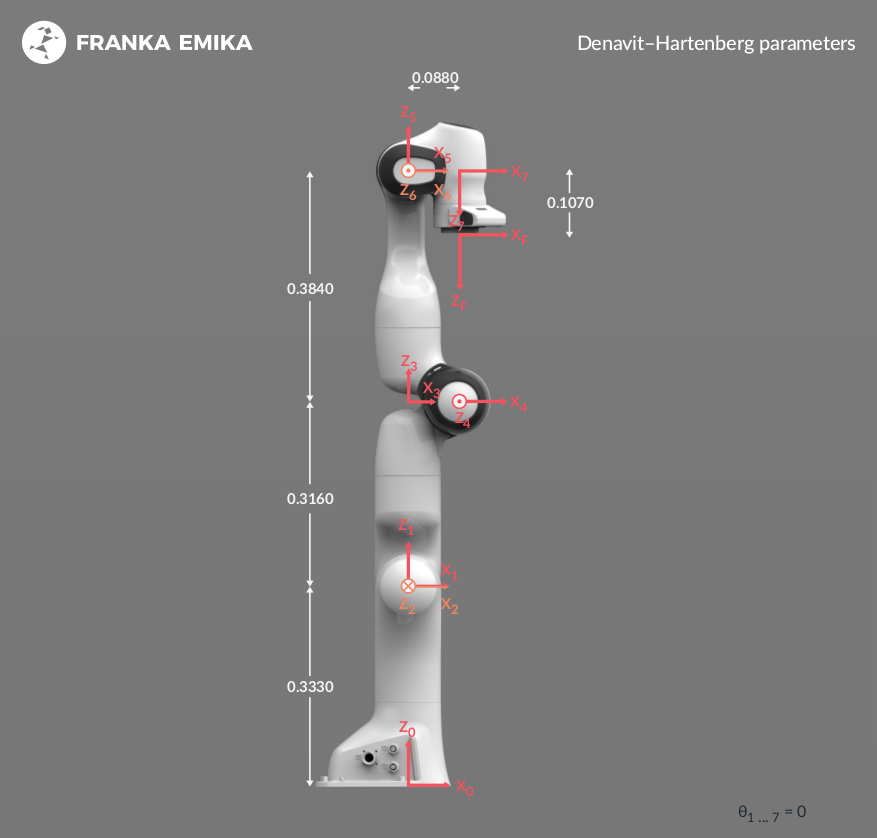
\includegraphics[width=\textwidth]{dh-diagram.png}
	\caption{\label{fig:robot_spec}Robot Specifications}
\end{figure}
\begin{figure}
	\centering
	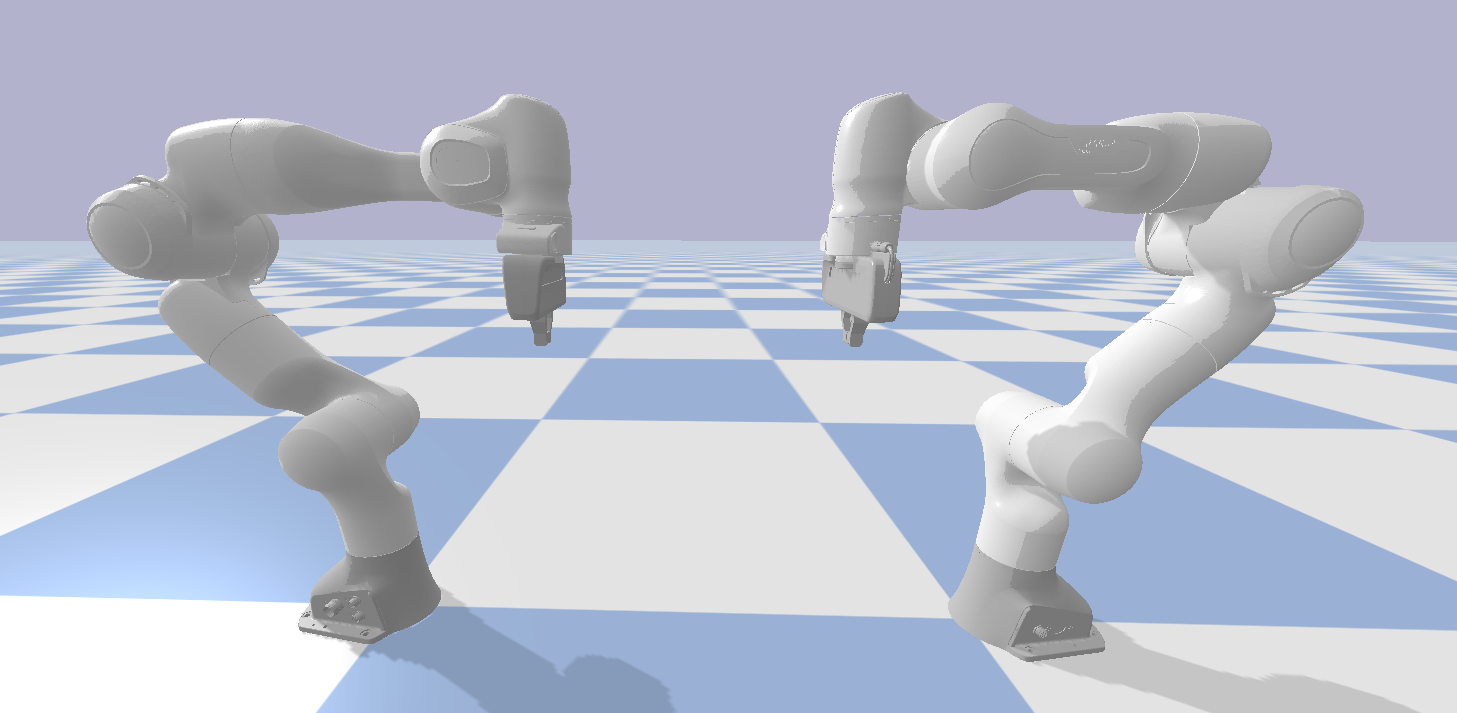
\includegraphics[width=0.6\textwidth]{initial_position.png}
	\caption{\label{fig:1}Initial position of the robots}
\end{figure}
%\begin{figure}
%	\centering
%	\includegraphics[width=\textwidth]{Diapositiva2.JPG}
%	\caption{\label{fig:2} E-E frame and Tool frame of Left Arm}
%\end{figure}
\begin{figure}
	\centering
	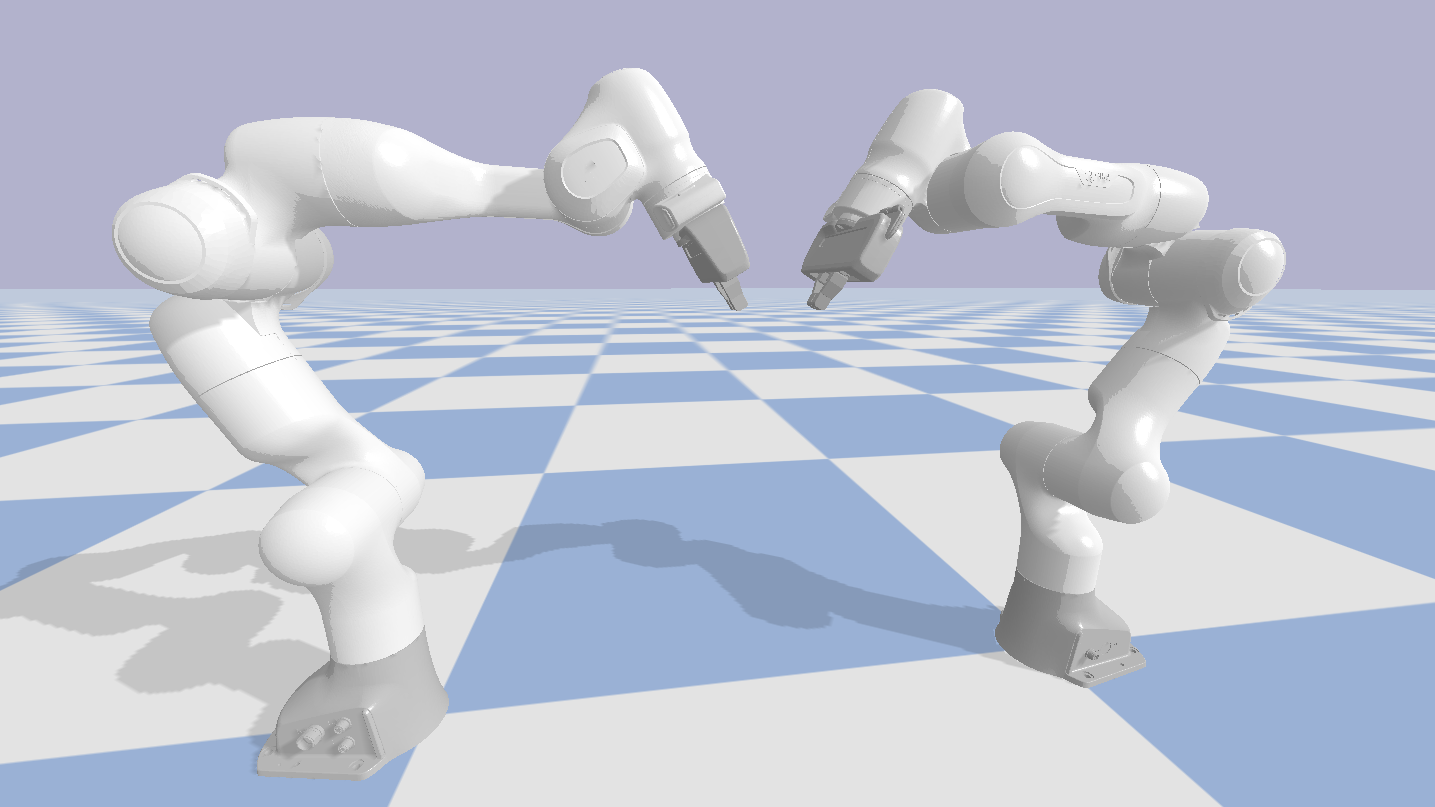
\includegraphics[width=0.6\textwidth]{grasping_position.png}
	\caption{\label{fig:3}Relative orientation at the grasping position}
\end{figure}

In this exercise it is required to perform a bimanual manipulation by implementing the task priority algorithm considering two manipulators as a single robot. The manipulator adopted for this assignment is the Franka Panda by Emika (see Figure \ref{fig:robot_spec})). A simulation in python is provided, in order to visualize the two robots and test your Matlab implementation.

\begin{enumerate}
	\item The transformations between the world and the base of each robot must be computed knowing that: 
	\begin{enumerate}
		\item The left arm base coincides with the world frame.
		\item The right arm base is rotated of $\pi$ w.r.t. z-axis and is positioned 1.06 m along the x-axis and -0.01 m along the y-axis.
		
	\end{enumerate}

	\item The transformation from each base to the respective end-effector is given in the code and is retrieved from the URDF model thanks to the \textit{Robotic System Toolbox} of Matlab.
	
	\item Then, define the tool frame for both manipulators; the tool frames must be placed at 21.04 cm along the z-axis of the end-effector frame and rotated with an angle of -44.9949 deg around the z-axis of the end-effector.
	
	\item Implement a ``move to'' action that includes the joint limits task.
	
	
	\item The first phase foresees to move the tool frame of both manipulators to the grasping points, by implementing  a ``move to'' action and its corresponding tasks. Define the goal frames for each manipulator such that their origin corresponds to the grasping points. \textbf{HINT}: the position of the grasping points can be computed by knowing the origin of the object frame $^{w}\textrm{O}_{o}$ and the object length $l_{obj}$. The goal orientation of the tool frames is obtained by rotating the tool frames 30 deg around their y-axis; the manipulators should reach the configuration depicted in Figure \ref{fig:3}. 
	

	\begin{equation}
		^{w}\textrm{O}_{o} = [0.5, 0, 0.59];
	\end{equation}
	\begin{equation}
		l_{obj} = 10\,  \text{(cm)}.
	\end{equation}

	\item During this phase of the mission, the following safety tasks must be implemented: \textit{end-effector minimum altitude} and \textit{joint limits}. The joint limits specifications can be found in the datasheet of the robot. The minimum altitude from the table should be 15 cm. 
\end{enumerate}


Once the manipulators reach the grasping points, the second phase of the mission should start. Now, implement the Bimanual Rigid Grasping Constraint task to carry the object as a rigid body. 
\begin{enumerate}
	\item Define the object frame as a rigid body attached to the tool frame of each manipulator. \textbf{HINT:} Compute this quantity after reaching the grasping point.
	\item Define the rigid grasp task.
	\item Then, move the object to another position while both manipulators hold it firmly, e.g. $ ^{w}\textrm{O}_{g} = [0.65, -0.35, 0.28]^{\top}(m)$
	\item Note that the transition for the \textit{Bimanual Rigid Constraint} should be a binary one, i.e., without smoothness. This is the nature of the constraint, i.e., either it exists or not. Modify the \emph{ActionTransition} script seen during the class to take into account the different nature of this task (a constraint one).
	
	
\end{enumerate}
 
Once the object has been moved to the required position you have to implement a final phase of the mission in which the joint velocities are set to zero, and every action is deactivated except for the minimum altitude task.

Repeat the simulation, using a goal position or by changing the grasping in such a way that one of the two manipulators activates multiple safety tasks, to stress the constraint task.

\subsection{Q1: Report the unified hierarchy of tasks used and their priorities in each action.}


Actions :\\ 

$\mathcal{A}_{1}$ - Move-to.


$\mathcal{A}_{2}$ - Co-operative move-to

$\mathcal{A}_{3}$ - Halt manipulator


\begin{table}[htb]
	\label{tbl:actions_tables}
	\begin{center}
		\footnotesize
		\begin{tabular}{cccccc}
			\toprule		
			Task & Type & $\mathcal{A}_{1}$ & $\mathcal{A}_{2}$  & $\mathcal{A}_{3}$  \\
			\midrule
			Joint limits                      & I & 1 & 1 &  \\
			\hdashline
			Minimum Altitude						& I & 2& 2 & \\
			\hdashline 
			Bimanumial rigid grasping constraint					& E & & 3 & \\
			\hdashline
			Move-To						& E & 3 & 4& \\ 
			%\hdashline 
			%\hdashline 
			%Position Control 						& E & & & & 4 \\ 
			
			\bottomrule
		\end{tabular}
	\end{center}
\caption{Example of actions/hierarchy table: A number in a given cell represents the priority of the control task (row) in the hierarchy of the control action (column). The type column indicates whether the objective is an equality (E) or inequality (I) one.}
\end{table}
\noindent
Task Defintions\\
Joint limits - This is safety task to constraint the each joints of the manipulator , which is responsible to maintain the joint angle in its range.\\
Minimum Altitude -  
This is the safety task where the tool of the manipulator keeps the minimum distance from the ground. \\
Bimanual rigid grasping constrain - In this task we constraint our robot to act together. \\
Move to - this task the manipulator move to the desired position 


\subsection{Q2: What is the Jacobian relationship for the Joint Limits task? How was the task reference computed?}


\subsection{Q3: What is the Jacobian relationship for the Bimanual Rigid Grasping Constraint task? How was the task reference computed?}

\subsection{Q4: Comment the behaviour of the robots, using relevant plots. In particular, show the difference (if any) between the desired object velocity, and the velocities of the two end-effectors in the two cases.}

\clearpage

\section{Exercise 3: Cooperative manipulation}
In this exercise, it is required to perform cooperative manipulation by implementing the task priority algorithm considering the two Franka Panda manipulators as two distinct robots. 

\begin{enumerate}
	
\item The first phase foresees to move the tool frames to the grasping points, by implementing the ``move to'' action for both manipulators. \textbf{Please note: each manipulator has his own Task Priority Inverse Kinematic Algorithm}. Define the goal frames for each manipulator such that their origin corresponds to the grasping points. \textbf{HINT}: the position of the grasping points can be computed by knowing the origin of the object frame $^{w}\textrm{O}_{o}$ and the object length $l_{obj}$. The goal orientation of the tool frames is obtained by rotating the tool frames 20 deg around their y-axis.

\begin{equation}
	^{w}\textrm{O}_{o} = [0.5, 0, 0.59]^{\top}(m);
\end{equation}
\begin{equation}
	l_{obj} = 6\,  \text{(cm)}.
\end{equation}

During this phase of the mission, the following safety tasks must be implemented: \textit{end-effector minimum altitude} and \textit{joint limits}. The joint limits specifications can be found in the datasheet of the robot. The minimum altitude from the table should be 15 cm. 

\item Once the manipulators reach the grasping points the second phase of the mission should start. Implement the \textit{Cooperative Rigid Constraint} task to carry the object as a rigid body. 
\begin{enumerate}
	\item Define the object frame as a rigid body attached to the tool frame of each manipulator. 
	\item Define the rigid grasp task. 
	\item You have to move the object to another position while both manipulators hold it firmly. The desired object goal position is
	\begin{equation}
		^{w}\textrm{O}_{g} = [0.60, 0.40, 0.48]^{\top}(m)
	\end{equation}
	\item Compute the \textit{non-cooperative} object frame velocities. \textbf{HINT:} Suppose manipulators communicate ideally and can exchange the respective end-effector velocities
	\item Apply the coordination policy to the \textit{non-cooperative} object frame velocities.
	\item Compute the \textit{cooperative} object frame velocities.
\end{enumerate}

Note that the transition for the \textit{Cooperative Rigid Constraint} should be a binary one, i.e., without smoothness. This is the nature of the constraint, i.e., either it exists or not. Modify the \emph{ActionTransition} script seen during the class to take into account the different nature of this task (a constraint one).

\item Once the object has been moved to the required position you have to implement a final phase of the mission in which the joint velocities are set to zero, and every action is deactivated except for the minimum altitude task.
\end{enumerate}

 Again, test it twice, once with the provided (reachable) goal, and then with a goal or with a different grasp configuration that triggers the activation of multiple joint limits or a joint limit and minimum altitude by one manipulator. The idea is that this second position should trigger the cooperation policy (i.e., the cooperative velocity should be different than the original desired object velocity).

\subsection{Q1: Report the unified hierarchy of tasks used and their priorities in each action, and report clearly the actions used in the two phases of the cooperation algorithm.}

\subsection{Q2: Comment the behaviour of the robots, using relevant plots. In particular, make sure there are differences between the desired object velocity and the non-cooperative Cartesian velocities at least in one simulation. Show also how the cooperative velocities of the two end-effectors behave.}

%\begin{figure}[t]
%	\centering
%	\subfloat[]{\includegraphics[height=7cm]{trident.jpg}}\label{fig:trident}
%	\subfloat[]{\includegraphics[height=7cm]{maris.jpg}}\label{fig:maris}
%	\caption{(a) TRIDENT UVMS (b) MARIS UVMS.}\label{fig:uvms_examples}
%\end{figure}


		
%		\begin{figure}[b]
%			\centering
%			\subfloat[]{\frame{\includegraphics[keepaspectratio,height=3cm]{trident1.eps}}} 
%			\subfloat[]{\frame{\includegraphics[keepaspectratio,height=3cm]{trident2.eps}}}
%			\subfloat[]{\frame{\includegraphics[keepaspectratio,height=3cm]{trident3.eps}}}
%			\subfloat[]{\frame{\includegraphics[keepaspectratio,height=3cm]{trident4.eps}}}
%			\caption{Sequence of snapshots taken from the onboard camera during the TRIDENT final experiments.}
%			\label{fig_tri_trial_maiorca_img}
%		\end{figure}
\clearpage


\end{document}


